%% 이 파일은 서울대학교 산업공학과 학위논문 양식을 정의하기 위해 아래 원저자, 1차 수정자, 
%% 서울대학교 산업공학과 데이터마이닝연구실에서 수정판 파일을 
%% 서울대학교 건설환경공학부 학위논문 형식에 맞춰 재수정한 파일입니다. (2021년 03월)
%% 원저자: zeta709 (zeta709@gmail.com) 
%% 1차 수정자: 서울대학교 데이터마이닝연구실 
%% 최종 수정자: 서울대학교 건설환경공학부 기후변화적응 수자원연구실 김기주 (gijoo-kim@naver.com) 

\RequirePackage{fix-cm} 

% 옵션 수정 가능 
% oneside/twoside : 단면 인쇄, 양면 인쇄 
% openright : 챕터가 홀수쪽에서 시작
% draft, final,etc....
\documentclass[oneside, phd]{snuthesis_utf8_eng}

%%%%%%%%%%%%%%%%%%%%%%%%%%%%%%%%%%%%%%%%
%% 목차 양식을 변경하는 코드
%% subfigure (subfig) package 사용 여부에 따라
%% tocloft의 옵션을 다르게 지정해야 한다.
%\usepackage[titles,subfigure]{tocloft} % when you use subfigure package
\usepackage[titles]{tocloft} % when you don't use subfigure package
%\usepackage{subfig}
\usepackage{amsmath,amssymb,amsthm,kotex,color}
\usepackage{tikz}
\usetikzlibrary{shapes,arrows}
\usepackage[]{algpseudocode,algorithm,algorithmicx}
\usepackage{setspace}
\usepackage{array}
\usepackage{romanbar}
\usepackage{pgfplots}
\usepackage{caption}
\usepackage{subcaption}
\usepackage{booktabs, multirow}
\usepackage{natbib}
\usepackage{threeparttable}
\usepackage{multirow}
\usepackage{rotating}
\usepackage{comment}
%\usepackage{indentfirst}\setlength\parindent{2em}

\usepackage{newtxtext,newtxmath}
\newcommand{\killpunct}[1]{}
\usepackage{lscape}


\makeatletter % don't delete me
\renewcommand\cftchappresnum{Chapter~}
\renewcommand\cftfigpresnum{Figure~}
\renewcommand\cfttabpresnum{Table~}
\renewcommand{\algorithmicforall}{\textbf{foreach}}

\newtheorem{theorem}{Theorem}[chapter]
\newtheorem{lemma}[theorem]{Lemma}
\newtheorem{proposition}[theorem]{Proposition}
\newtheorem{corollary}[theorem]{Corollary}
\newtheorem{definition}[theorem]{Definition}
\newtheorem{Proposition}{Proposition}
\newtheorem{remark}{Remark}[chapter]
\newtheorem{example}{Example}[chapter]
\usepackage[pdftex,bookmarks=true]{hyperref}

\makeatother % don't delete me
\newlength{\mytmplen}
\settowidth{\mytmplen}{\bfseries\cftchappresnum\cftchapaftersnum}
\addtolength{\cftchapnumwidth}{\mytmplen}
\settowidth{\mytmplen}{\bfseries\cftfigpresnum\cftfigaftersnum}
\addtolength{\cftfignumwidth}{\mytmplen}
\settowidth{\mytmplen}{\bfseries\cfttabpresnum\cfttabaftersnum}
\addtolength{\cfttabnumwidth}{\mytmplen}
%% 목차 양식을 변경하는 코드 끝
%%%%%%%%%%%%%%%%%%%%%%%%%%%%%%%%%%%%%%%%

%%%%%%%%%%%%%%%%%%%%%%%%%%%%%%%%%%%%%%%%
%% 다른 패키지 로드
%% http://faq.ktug.or.kr/faq/pdflatex%B0%FAlatex%B5%BF%BD%C3%BB%E7%BF%EB
%% 필요에 따라 직접 수정 필요
\ifpdf
	% \input glyphtounicode\pdfgentounicode=1 %type 1 font사용시
	%\usepackage[pdftex,unicode]{hyperref} % delete me
	%\usepackage[pdftex]{graphicx}
	%\usepackage[pdftex,svgnames]{xcolor}
\else
	%\usepackage[dvipdfmx,unicode]{hyperref} % delete me%
	%\usepackage[dvipdfmx]{graphicx}
	%\usepackage[dvipdfmx,svgnames]{xcolor}
\fi
%%%%%%%%%%%%%%%%%%%%%%%%%%%%%%%%%%%%%%%%
%
%% \title : 22pt로 나오는 큰 제목
%% \title*: 16pt로 나오는 작은 제목

\title{Sample Title}
\title*{제목 예시}
\titlen{}

\author{Ab Abc~Kim}
\author*{가가가} % Same as \author.
\authorn{가~가~가}
\phonenumber{010-1234-1234}
\studentnumber{2000-00000}
\advisor{Gil Dong~Hong}
\advisor*{홍길동}
\advisorn{홍~길~동}
\graddate{2022~년~~2~월}
\submissiondate{2021~년~~11~월}
\submissiondaten{2021~년~~11~월~~1~일}
\approvaldate{2021~년~~12~월}

\committeemembers%
{김 원 장}%
{홍 길 동}%
{박 위 원}%
{최 위 원}%
{한 위 원}%

%% Length of underline
\setlength{\committeenameunderlinelength}{5cm}

\pgfplotsset{compat=1.17} 
\begin{document}
%  \pagenumbering{Roman}
%  \makefrontcover
%  \makeapproval

% %agreement page
% \cleardoublepage
% \makeagreement
% \cleardoublepage
% \pagenumbering{roman}
% \keyword{Production planning, Optimization, Industrial engineering}
% \begin{abstract}
% In this thesis, we consider a production planning problem arising in real-world industry. We propose mathematical optimization techniques for solving the problem. We verify that the proposed solution approaches are more effective than existing methods.
% \end{abstract}

%목차 구성
\pagenumbering{roman}

\newpage
\addcontentsline{toc}{chapter}{\contentsname}
\tableofcontents
\cleardoublepage

\newpage
\addcontentsline{toc}{chapter}{\listtablename}
\listoftables
\cleardoublepage

\newpage
\addcontentsline{toc}{chapter}{\listfigurename}
\listoffigures
\cleardoublepage


% \centering \textbf{List of Symbols} 

% \textbf{Latin uppercase}

% \begin{tabular}{@{}ll}
% $\lambda$ & 1-Dimension Advection-Dispersion Equation \\
% BTC & Breakthrough Curve \\
% DR & Discrepancy Ratio \\
% GA & Genetic Algorithm \\
% GP & Genetic Programming \\
% HTS & Hyporheic Transient Storage \\
% MGGP & Multi-Gene Genetic Programming \\
% MSE & Mean Squared Error \\
% MSL & Mean Sea Level \\
% OAT & One-At-a-Time \\
% OTIS & One-Dimensional Transport with Inflow and Storage\\
% PCR & Principal Components Regression\\
% RMSE & Root Mean Squared Error\\
% % RPCR & Robust Principal Components Regression\\
% RTD & Residence Time Distribution \\
% RWT & Rhodamine WT \\
% SC-SAHEL & Shuffled Complex-Self Adaptive EvoLution\\
% SCE-UA & Shuffled Complex Evolution-University of Arizona\\
% SI & Sensitivity Index\\
% STS & Surface Transient Storage \\
% TSM & Transient Storage Model\\
% VIF & Variance Inflation Factor \\
% \end{tabular}

% \cleardoublepage


\pagenumbering{arabic}
%%%%%%%%%%%%%%%%%%%%%%%%%%%%%%%%%%%%%%%%%%%%%%%%%%%%%%%%%CHAPTER 1%%%%%%%%%%%%%%%%%%%%%%%%%%%%%%%%%%%%%%%%%%%%%%%%%%%%%%%%%%%%%%%%%
\chapter{Introduction}\label{c1}
This is a sample sentence for testing in Chapter 1 of the dissertation. This is a sample sentence for testing in Chapter 1 of the dissertation. 

New paragraph starts like this, and citation with parenthesis as the following: \citep{bloschl:2019twenty}.
Citations without parenthesis as: \cite{bloschl:2019twenty}


\newpage
\section{Introduction-Section1}\label{s1.1}
Sample Text


\subsection{Introduction-Subsection1.1}
Sample Text


\subsection{Introduction-Subsection1.2}
Sample Text 


\subsection{Introduction-Subsection1.3}
Sample Text


\newpage
\section{Introduction-Section2}\label{s1.2}
Sample Text

Sample Enumerating looks like this:
\begin{enumerate}
\item[(a)] Enumerate Item 1
\item[(b)] Enumerate Item 2
\item[(c)] Enumerate Item 3
\end{enumerate}


Sample Table looks like this:
\begin{table}[h] \centering
\caption{Sample Table}
\begin{tabular}{c|c|c|c|c}
\toprule
Column 1 & Column 2 & Column 3 & Column 4 & Column 5 \\
\hline \hline
A & 1 & 2 & 3 & 4 \\
\hline
B & 1 & 2 & 3 & 4 \\
\hline
C & 1 & 2 & 3 & 4 \\
\hline
\end{tabular}\label{table:1} 
\end{table}

Refer to the above table as: Table \ref{table:1}.


\newpage
%%%%%%%%%%%%%%%%%%%%%%%%%%%%%%%%%%%%%%%%%%%%%%%%%%%%%%%%%CHAPTER 2%%%%%%%%%%%%%%%%%%%%%%%%%%%%%%%%%%%%%%%%%%%%%%%%%%%%%%%%%%%%%%%%%
\chapter{Methodology}\label{c2}
This is a sample sentence for testing in Chapter 2 of the dissertation. This is a sample sentence for testing in Chapter 2 of the dissertation.  

Sample Figure looks like this:

\begin{figure}[p]\centering \begin{center}
 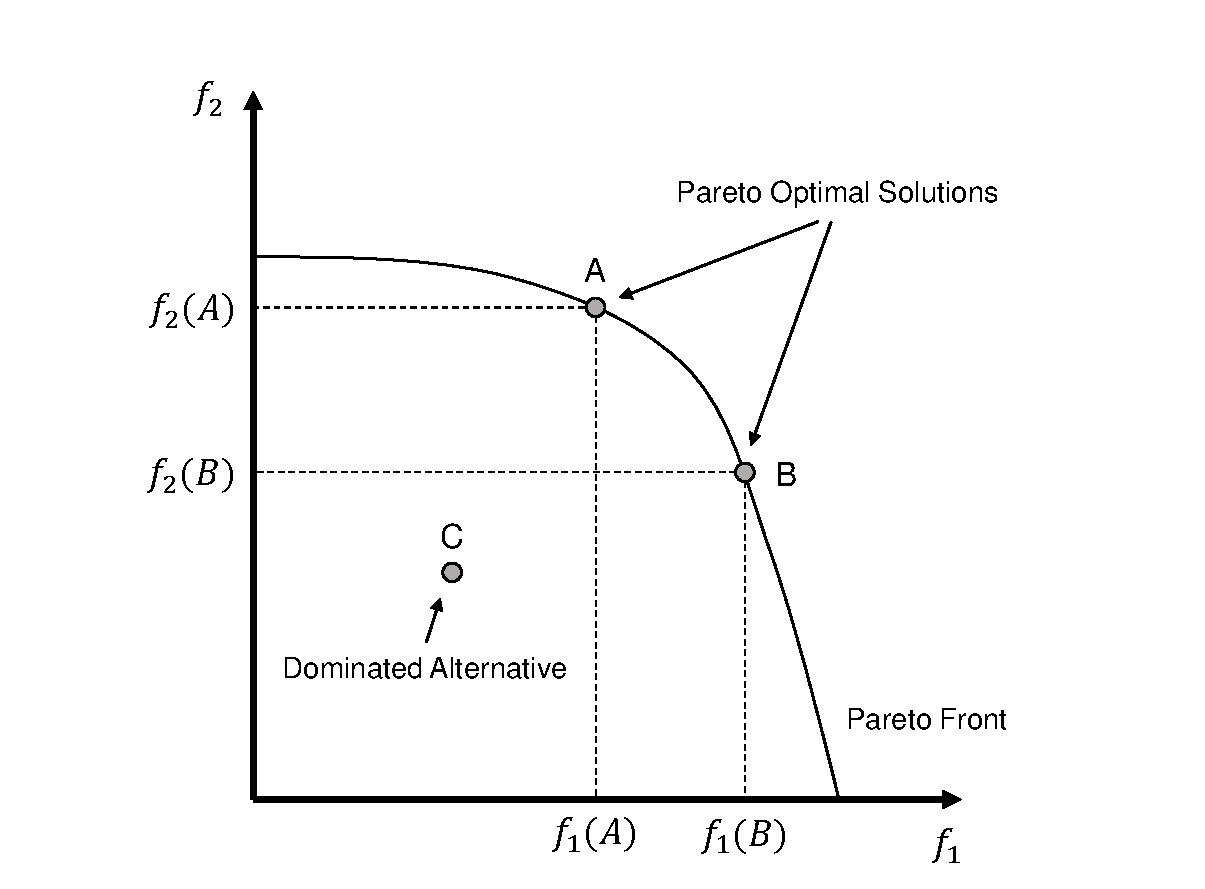
\includegraphics[scale=.50]{sample_fig.pdf}
 \end{center} \vfill
\caption{Sample Figure} 
\label{figure:1}
\end{figure}
\clearpage

Refer to the above figure as: Fig. \ref{figure:1}.


Sample Equation looks like this:
\begin{equation} \label{eq:1}
Z(\mathbf{x}) = \sum^{k}_{i=1} w_{i} f_{i}(\mathbf{x})
\end{equation}

Refer to the above equation as: Eq.~\ref{eq:1}.




%%%%%%%%%%%%%%%%%%%%%%%%%%%%%%%%%%%%%%%%%%%%%%%%%%%%%%%% BIBLIOGRAPHY %%%%%%%%%%%%%%%%%%%%%%%%%%%%%%%%%%%%%%%%%%%%%%%%%%%%%%%%%%%%%
\begin{bibpage}
\renewcommand{\bibname}{Bibliography}
\bibliography{ref_sample}
\bibliographystyle{ascelike-new} % Or any other style you like
\nocite{*}
\end{bibpage}

\end{document}